\section{$Re_{\tau}=2000$ simulation} 
The last simulation performed is carried out at $Re_{\tau}\approx2000$, which in terms of channel width and bulk velocity is approximately equivalent to $Re_{b}=100000$.\par
The bulk velocity is 24.3, $\alpha_{0}$ is 0.5 and $\beta_{0}$ is equal to 1.\par
The timestep is constant, with \emph{dt}=0.00001 and the simulation time is T=1. \par
The excessive resource requests lead us to perform a reduced simulation, able just to highlight the principal features of this $Re_{\tau}$. The simulation time, indeed, is reduced to a single non-dimensional units, however, in order to guarantee good results, we sampled the field every 0.001 steps, so that we can employ a 1000 fields to do the ensemble average.\\~\par
The grid employed in this simulation face 1000 points in the wall-normal direction, 4096 in the spanwise direction and 4096 points along the streamwise dimension. The mesh size is extremely huge, with more than 8 billions of points.\par
We reported a summary of the simulation configuration in table~\ref{table:2000}\\~\par

\begin{table}
\caption{Simulation data for $Re_{\tau}$=2000}
\begin{center}
\begin{tabular}{ccccccccccccc}
\toprule
$L_{x}$ & $L_{z}$ & $\delta$ & $nx$ & $nz$ & $ny$ & $\alpha_{0}$ & $\beta_{0}$ & $\Delta x^{+}$ & $\Delta z^{+}$ & $px$ & $dt$ & $T$\\
$4\pi$ & $2\pi$ & 1 & 4096 & 4096 & 1000 & 0.5 & 1 & 6.1  & 3 & 1 & 0.00002 & 1 \\
\bottomrule
\end{tabular}
\end{center}
\label{table:2000}
\end{table}


The disk space requirement raised approximately by a factor of 10, with 400GB of disk space needed per each field. This reason pushed us once again to rely in live post processing, instead of saving snapshots of the field.\\~\par

The statistics gained from the simulation are here presented.\par
We start from figure~\ref{loglaw:2000}, which report the law of the wall. Despite the graph is not perfect, during the simulation the data has shown a tendency to re-align with the theoretical behavior, characterized by $k=0.41$ and $B=5.2$. As consequence, towards the centerline, the velocity defect law is affected by fluctuations caused by the poor temporal resolution, as shown by the graph~\ref{velocity:defect:2000}. Despite these fluctuations, it is possible to see that the region subject to linearity has grown again \\~\par

\begin{figure}
\begin{center}
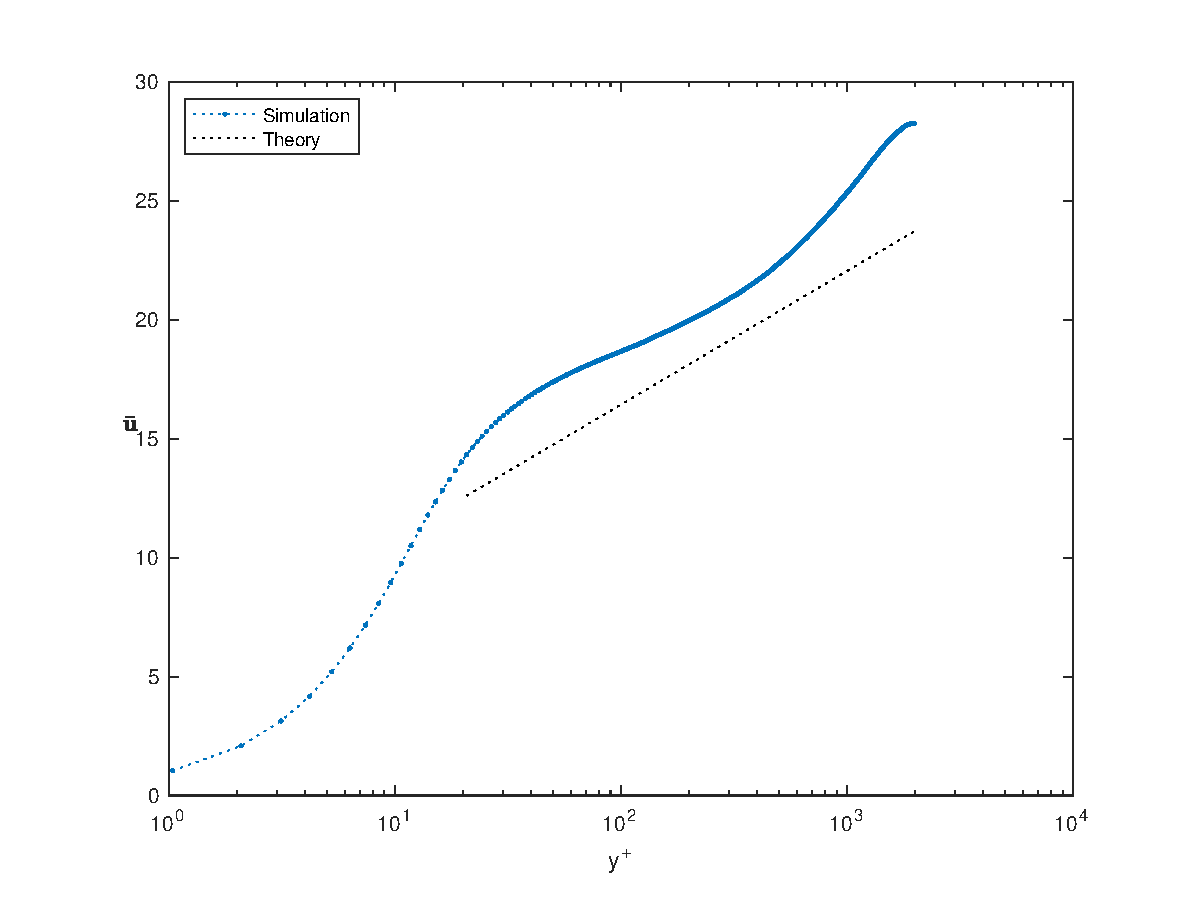
\includegraphics[scale=0.55]{grafici/loglaw_2000.eps}
\caption{$\bar{u}^{+}$ in the near wall region for a $Re_{\tau}=2000$ simulation}
\label{loglaw:2000}
\end{center} 
\end{figure}

\begin{figure}
\begin{center}
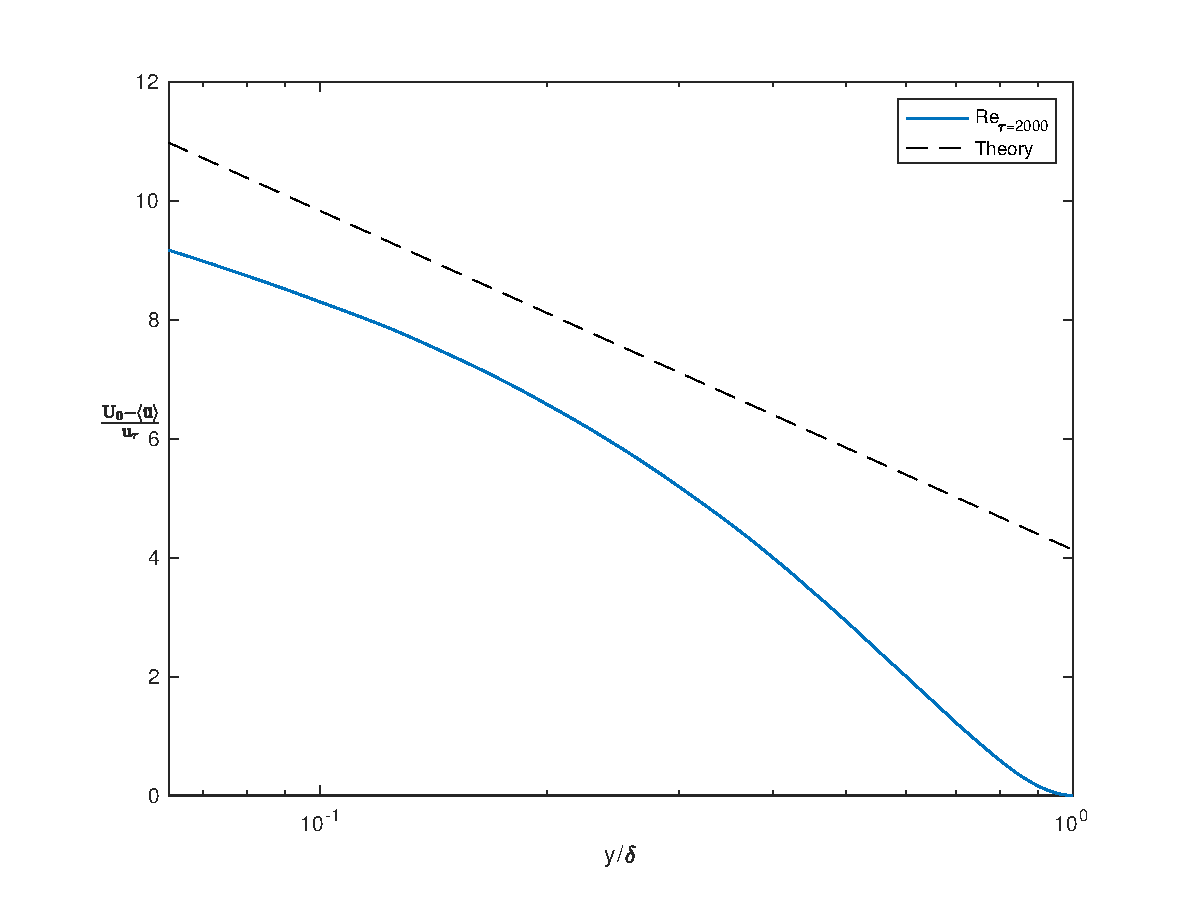
\includegraphics[scale=0.55]{grafici/velocity_defect_2000.eps}
\caption{Velocity defect for a $Re_{\tau}=2000$ simulation}
\label{velocity:defect:2000}
\end{center} 
\end{figure}

In figure~\ref{budget:2000} we reported the \emph{rms} fluctuations, normalized by the $u_{\tau}^{2}$, jointed with the TKE distribution. The first difference we can see by comparing this graph with the others is related to the peak values, which have incremented again, in line with our expectations for a more turbulent flow. \par
This time we can see that, followed by the raise in peak values, the spanwise and streamwise fluctuations exhibit a wider basement, with more energy   associated to those distances from the wall. This fact is partially due to the reduced lengthscale of this simulation with respect to the previous.\par
However, as the lens magnify, despite of the higher $Re_{\tau}$, the turbulence still tend to exhibit itself as a bi-dimensional phenomena close to the wall, exactly what happens also for \emph{low Reynolds} simulations.\par

Reaching the centerline the \emph{rms} terms and the TKE curve tends to align with the values of the $Re_{\tau}=1000$ simulation.\\~\par

\begin{figure}
\begin{center}
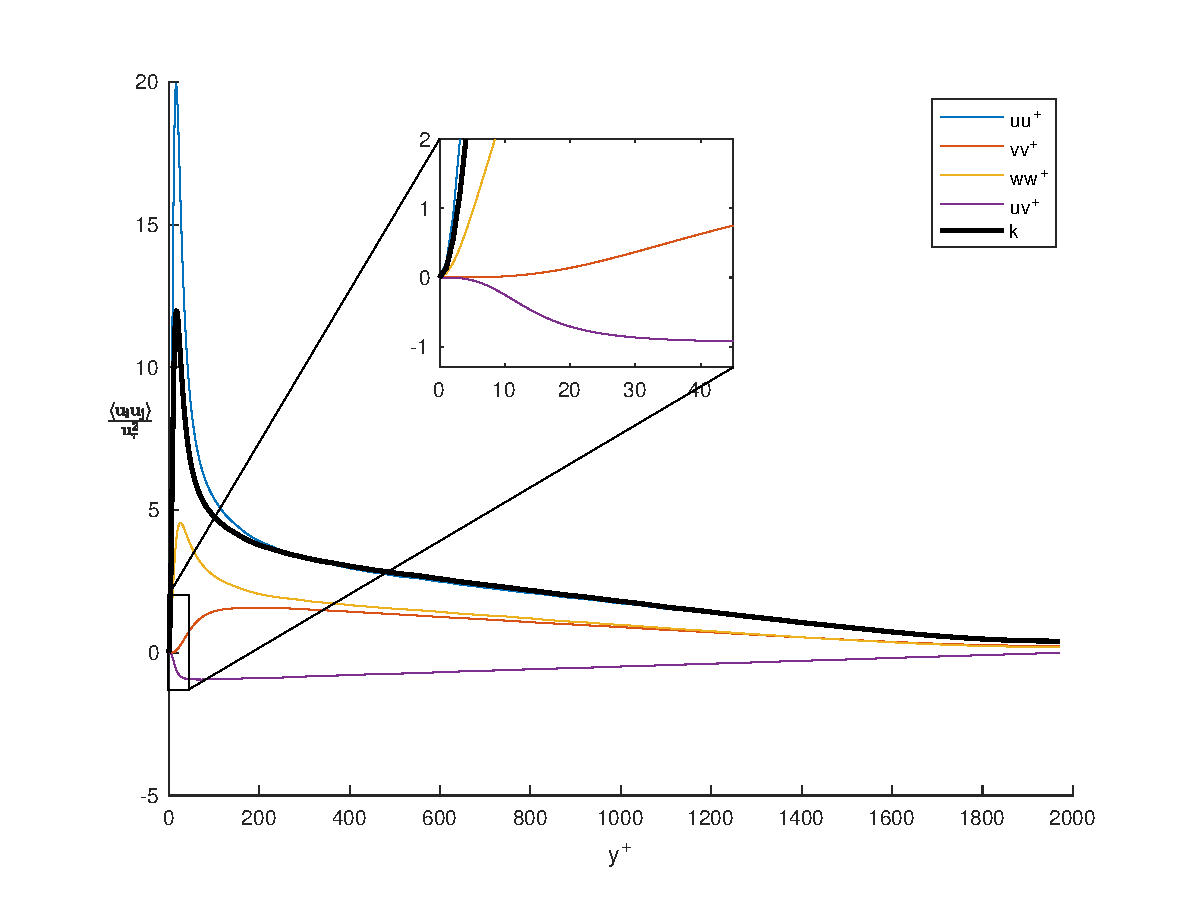
\includegraphics[scale=0.55]{grafici/budget+k_2000.eps}
\caption{\emph{rms} terms for a $Re_{\tau}=2000$ simulation}
\label{budget:2000}
\end{center} 
\end{figure}


The raise in Reynolds number modified the fluctuations distribution with a generalized upward shift, as figure~\ref{rms:2000} report, pushing the peaks towards higher values, with the peaks coordinate remaining approximately constant. The knee tends to move rightward for all the \emph{rms} terms, towards the centerline. Also the outer-cycle peaks tend to exhibit an upward shift, however it results to be lower than the previous boost.\\~\par

\begin{figure}
\begin{center}
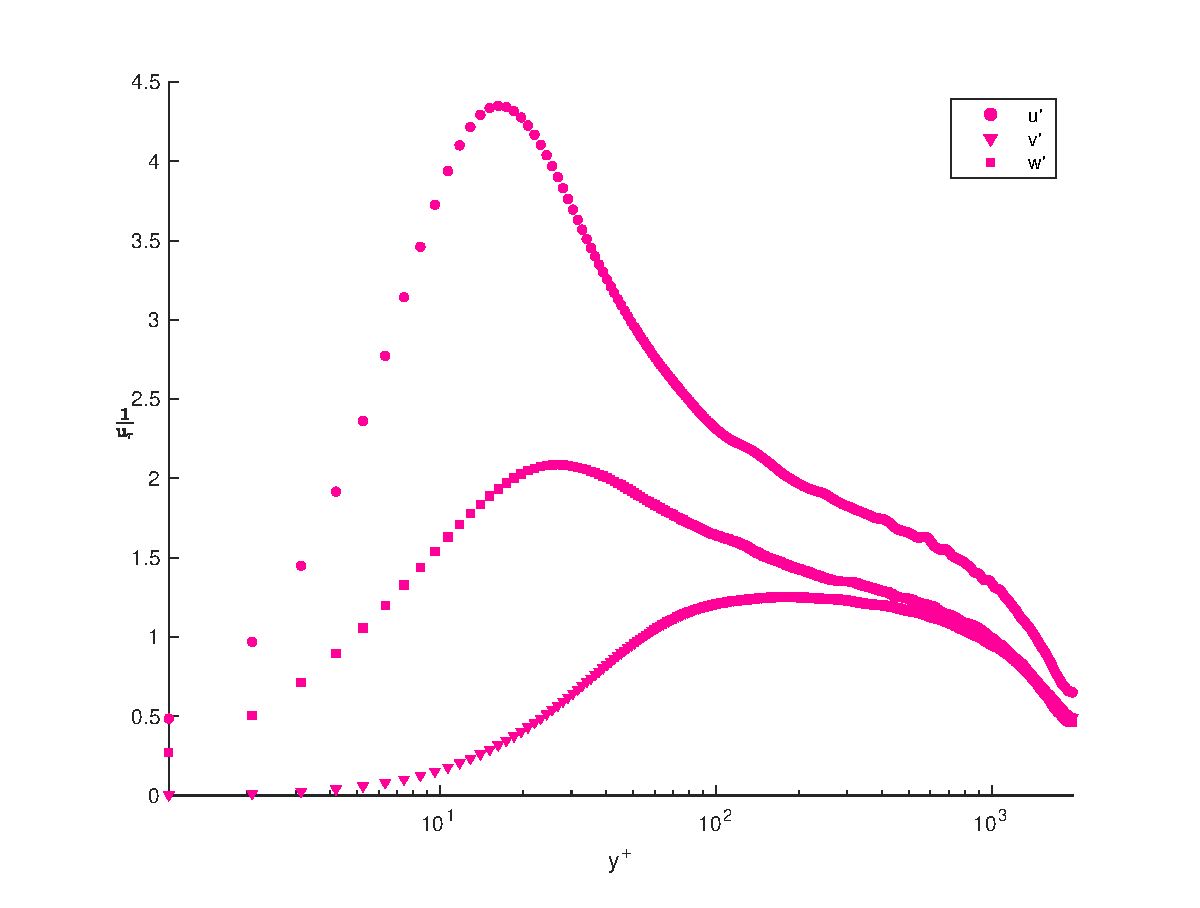
\includegraphics[scale=0.55]{grafici/rms_2000.eps}
\caption{\emph{rms} behavior on a $Re_{\tau}=2000$ simulation}
\label{rms:2000}
\end{center} 
\end{figure}

\begin{figure}
\begin{center}
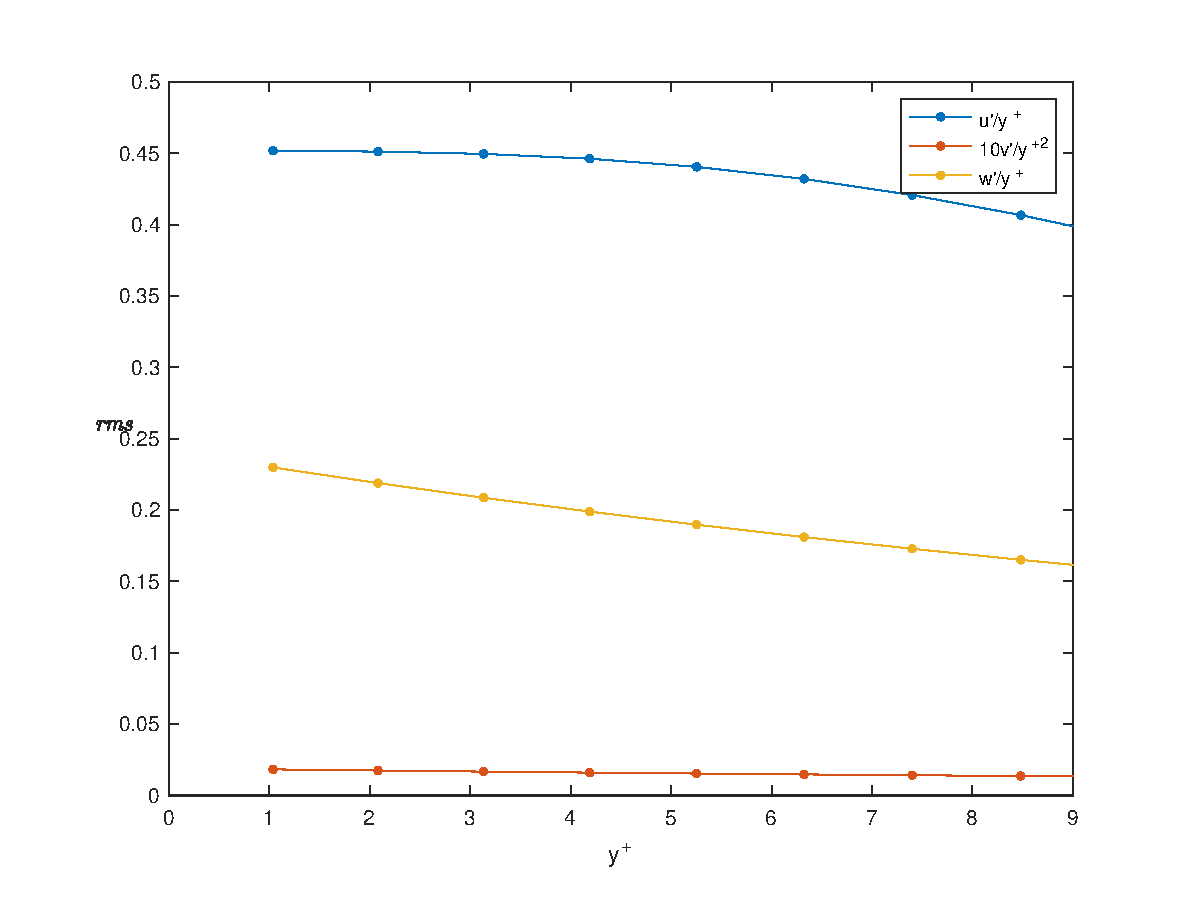
\includegraphics[scale=0.55]{grafici/wall_rms_2000.eps}
\caption{Normalized \emph{rms} close to the wall for a $Re_{\tau}=2000$ simulation}
\label{wall:rms:2000}
\end{center} 
\end{figure}

The streamwise and spanwise \emph{rms} terms tends to be higher since they leave the wall, this can be caught by comparing figure~\ref{wall:rms:2000} with figure~\ref{wall:rms:1000}. As can be recovered from the plot, such curves exhibit a linear growth for a wider range of wall coordinates, with respect to previous simulations. \par
The wall-normal fluctuation develops perfectly as $y^{+2}$ and its starting value is lower than the ones in previous simulations.\\~\par


For what concern about the \emph{production} term of the turbulent kinetic energy, according to figure~\ref{tke:prod:2000}, we can see that there are no changes to the profile, with the peak which remains near $y\approx12$. \\~\par

The normalized total shear stress profile is presented in figure~\ref{stresses:2000}. The graph exhibit the typical profile, with the Reynolds stresses that grows immediately and reach their peak before $y^{+}\approx 100$. \par
The crossing point between the viscous stress and Reynolds ones is still around $y\approx12$. This will be shown in the next chapter with an higher level of detail.


\begin{figure}
\begin{center}
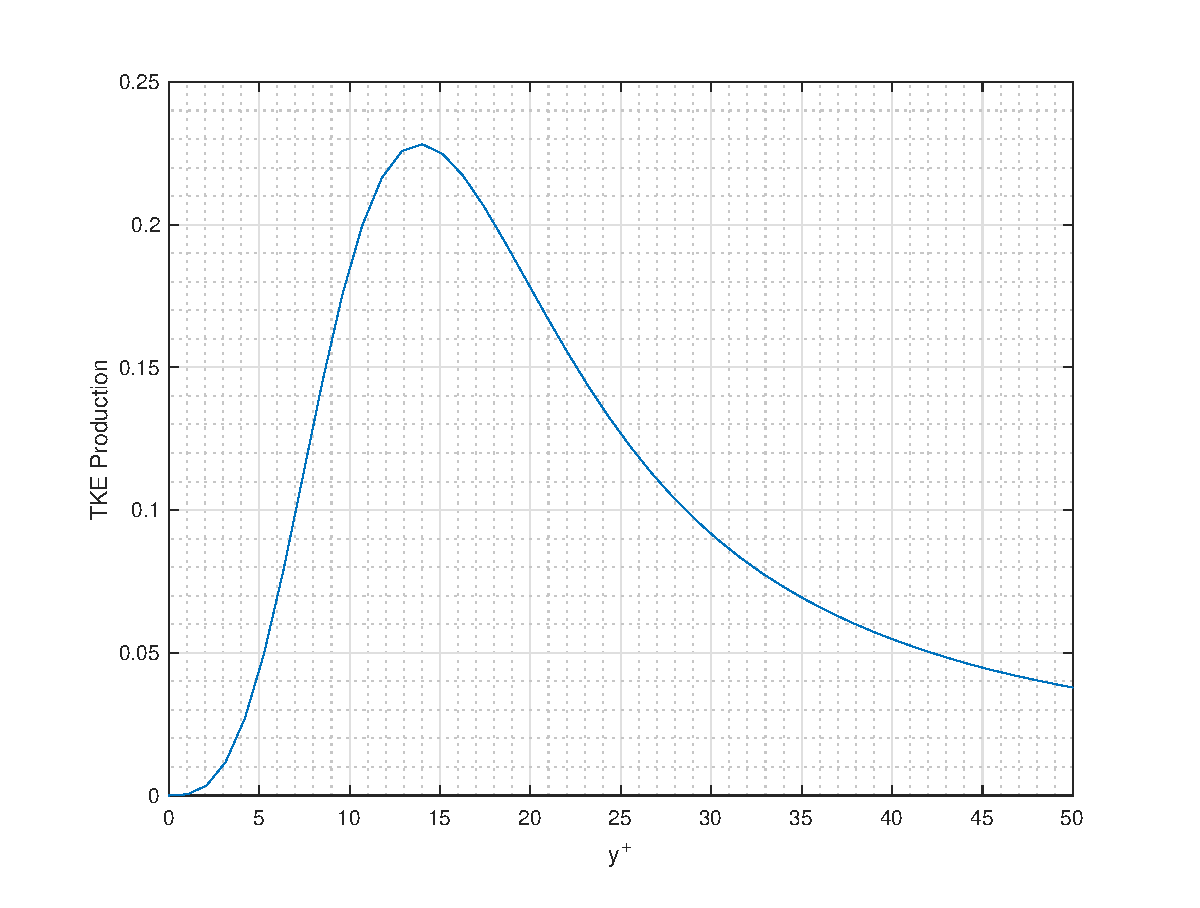
\includegraphics[scale=0.55]{grafici/tke_prod_2000.eps}
\caption{Production term of the TKE eq. for a $Re_{\tau}=2000$ simulation}
\label{tke:prod:2000}
\end{center} 
\end{figure}

\begin{figure}
\begin{center}
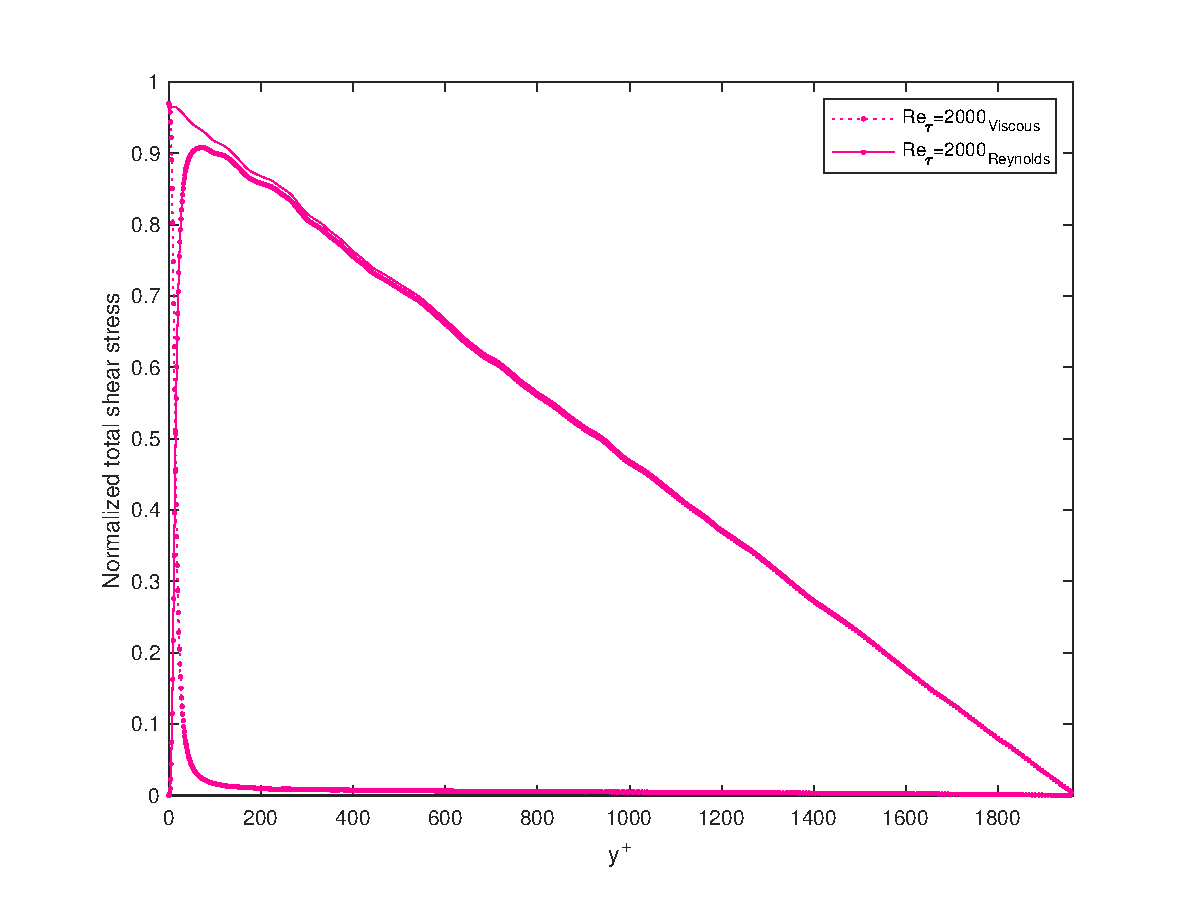
\includegraphics[scale=0.55]{grafici/stresses_2000.eps}
\caption{Normalized total shear stress for a $Re_{\tau}=2000$ simulation}
\label{stresses:2000}
\end{center} 
\end{figure}